%%%%%%%%%%%%%%%%%%%%%%%%%%% Figure 3 Godafoss %%%%%%%%%%%%%%%%%%%%%%%%%%%%%%%
\begin{figure}[t]
 \begin{center}
  \begin{pspicture}(0,0)(15,6.5)
% Include graphs
   \rput[bl]( 0.0,0.0){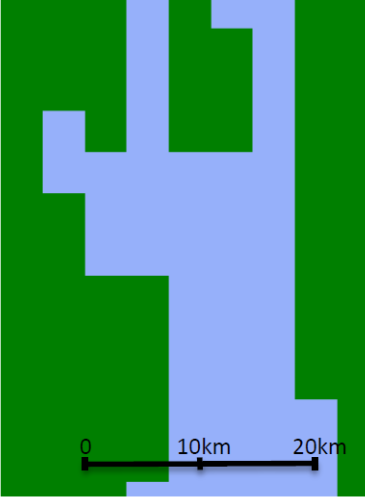
\includegraphics[height=6.5cm]{Midfjord_N4_grid}}
   \rput[b ]( 7.5,0.0){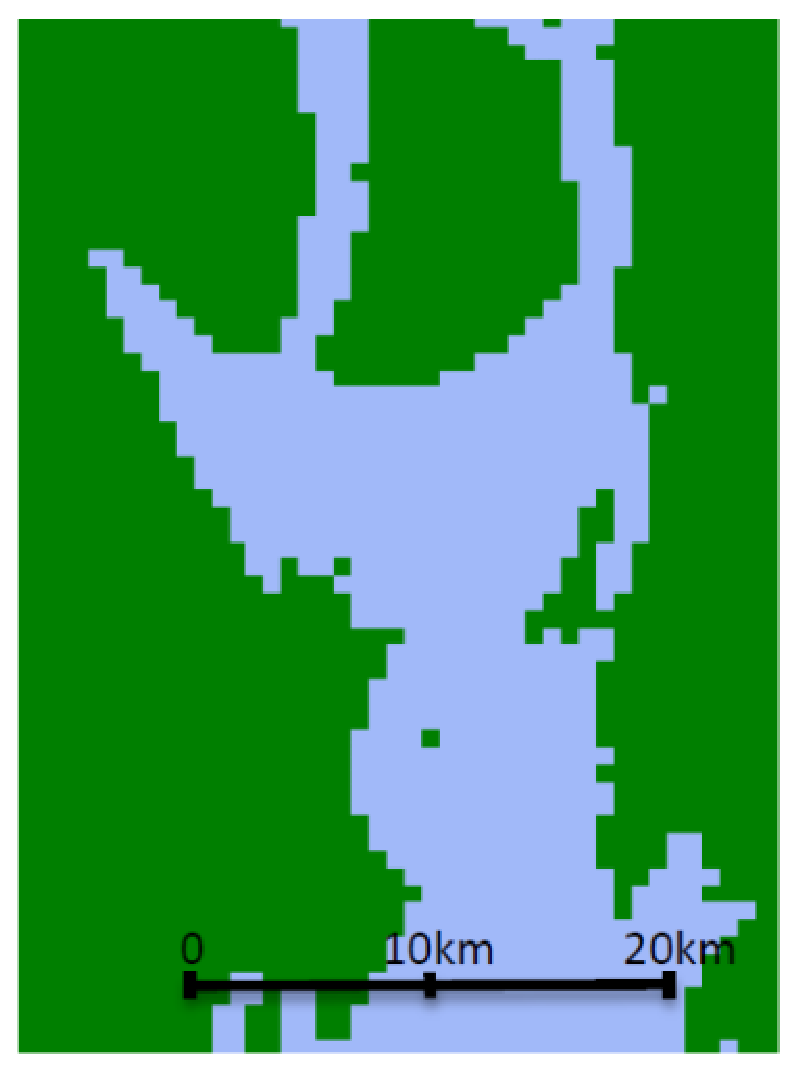
\includegraphics[height=6.5cm]{Midfjord_N800_grid}}
   \rput[br](15.0,0.0){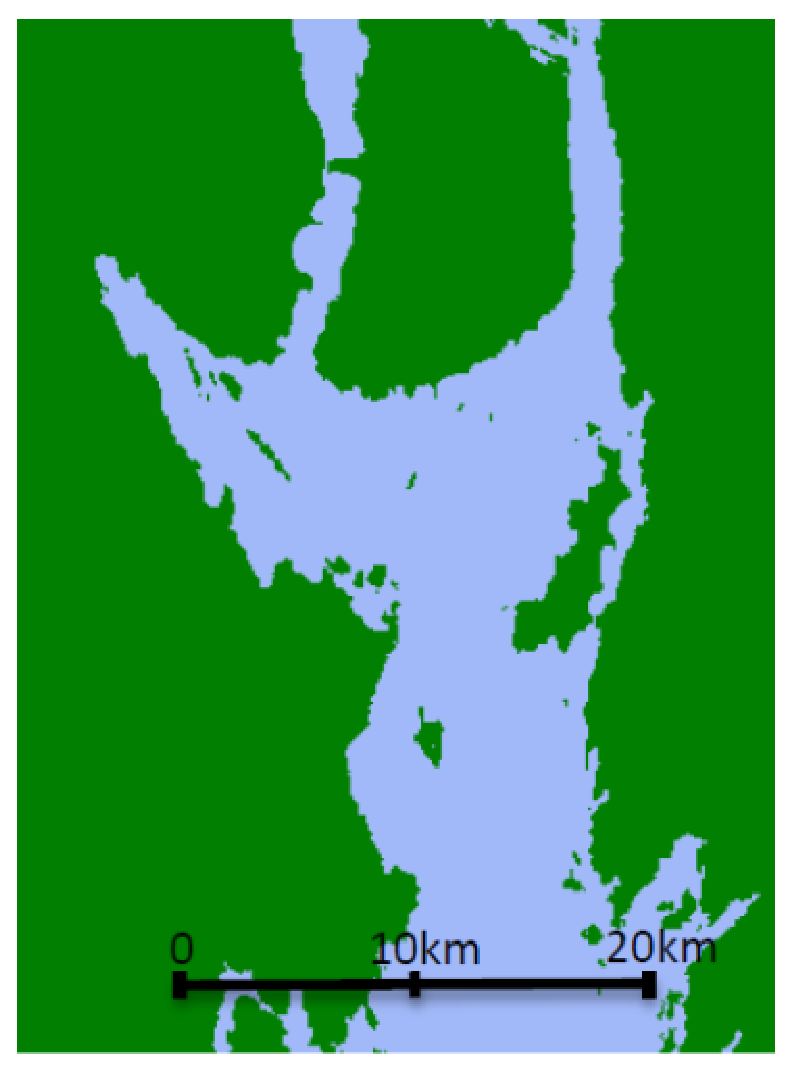
\includegraphics[height=6.5cm]{Midfjord_100m_grid}}
   \rput[bl]( 0.3,6.0){\large \textbf{a)}}
   \rput[b ]( 5.6,6.0){\large \textbf{b)}}
   \rput[br](10.9,6.0){\large \textbf{c)}}
  \end{pspicture}
  \caption{\small As Figure \ref{fig:resolution}, but zoomed in on Breidangen. To better reveal the grid the underlying map is not shown. (a) 4 km grid, (b) 800 m grid and (c) 100 m grid. Note that it takes a 100 m grid to properly resolve the many islands, narrow straits and channels present in the fjord. } 
  \label{fig:resolution_2}
 \end{center}
\end{figure}

